%!TEX root = ../../super_main.tex
\section{Server}
\label{sec:server}
The server, as seen in the top right part of \ref{fig:system_architecture}, both provides an Graphical User Interface (GUI) for the customers, and an Application Programming Interface (API) for the communication between the device and the server, such as upstream of snapshots from the devices of the participants or fetching campaign informations for the GUI on the device. 
\\\\
The server utilizes a web server technology, called NGINX, to serve dynamic content over the Hyper Text Transfer Protocol (HTTP). Furhtermore the server hosts a PostgreSQL database, which allows us to store the data collected from all the participants, as well as information regarding customers and campaigns.  
With these features the server is now able to facilitate the Laravel\footnote{https://laravel.com} web framework, which is a framework built on the model-view-controller (MVC) pattern. This allows us to route incoming requests and differentitate between requests from a device wanting JSON and requests from a customer using a browser. 

%!TEX root = ../../../super_main.tex
\subsection{Server Interface}
\label{sub:server_interface}
The interface from the clients to the server also needs to be considered. We chose to follow the REST principles \parencite{http_manden} and implement a RESTful API. This contributes to our architectures ability to handle an increasing amount of clients. The REST principles involve having a layered system with an uniform interface from the perspective of all devices regardless of how we choose to expand the capacity of the back end. This means that we can use modern technologies to handle load balancing and caching for web APIs and applications, allowing us to serve more users, without these changes being apparent on the client side. This will help scaling out to many servers, by balancing work to all available server instances, and scaling up by providing better performance on individual machines through caching. This effectively means that we can reduce the problem of scalability to implementing a proper RESTful interface. 
\\\\
The communication between the server and the client will be done over HTTP, and we will ensure that each resource, e.g. a campaign or a snapshot, will have a Unique Resource Identifier (URI). In our system we have need for storing three different kinds of resources on our server, namely campaigns, snapshots, and participants. The main object in our system is the campaign, and each other object will only exist in the system if it is somehow linked to a campaign, meaning that it makes sense to form the URI for these associated items as a part of a campaign. \tabref{tab:api_routes} shows the routes of the system that have something to do with retrieving these resources and the associated information (the first two routes), and joining and uploading snapshots (the last two routes). As seen in \tabref{tab:api_routes} all of these routes is prefixed with ``\mono{api}'' which is used to indicate that these routes will return a response in JSON-format.
\begin{table}[!htbp]
    \centering
    \begin{tabular}{|l|l|l|} 
        \hline
        \textbf{Name} & \textbf{Method} & \textbf{URI}                                  \\ \hline 
        \emph{show all} & \mono{GET }   & \mono{api/campaigns}                          \\ \hline 
        \emph{show one} & \mono{GET }   & \mono{api/campaigns/\{identifier\}}           \\ \hline 
        \emph{join}     & \mono{POST}   & \mono{api/campaigns/\{identifier\}/participants}\\ \hline 
        \emph{upload}   & \mono{POST}   & \mono{api/campaigns/\{identifier\}/snapshots} \\ \hline 
    \end{tabular}
    \caption{The routes that the client uses to send and get information to and from the server.}
    \label{tab:api_routes}
\end{table}
\FloatBarrier
The first two routes uses the \mono{GET} request method  to retrieve information regarding campaigns. The \emph{show all} route is requested from the device to return a list of identifiers, names and authors for all publicly available campaigns. The identifier from the request can be used using the \emph{show one} route, which return all the specifications of a specific campaign provided an identifier. The route captures the \mono{identifier} between the curly braces, provides it as a variable, which can be used to look up a record in our database. Assuming that a campaign with an id of 5 exists in the database, the route \mono{api/campaigns/5} would return a JSON response containing all details about this campaign. 
\\\\
The final two routes shown in \tabref{tab:api_routes} both uses the \mono{POST} request method, meaning that they are used for upload. The \emph{join} route is utilized when a participant, through the client application, joins a campaign, and the \emph{upload} route is used for uploading snapshots after participants have joined a campaign and are contributing to it. In the \emph{upload} and \emph{join} route the \mono{identifier} is also identifying a campaign, and the data, such as the device identifier for the \emph{join} route or the snapshot data for the \emph{upload} route, are stored in the body of the request. 
\\\\
Besides the routes for the Android client there also exist routes related to the user interface of the web application. These routes are not prefixed with ``\mono{api}'', and are used for creating and managing the campaigns in the system and retrieve information about the campaigns and their submitted snapshots. These routes are further described in \secref{sec:customer_interaction}. 

\subsubsection{Server Names}
\label{sub:server_names}

A problem that we have dealt with during the setup of the servers was that it was placed on the university. Problems arose when we wished to access the server from outside the university network. We had to request the network committee on AAU to gain access from the outside of the university. However, in doing this the we would have to utilize another IP to access the server from outside the university network. This would not have been a problem if the IP that was utilized to access the server outside the university network also worked when one was connected to the university network, however this was not the case. Furthermore, we also wanted two version of our web site and API: one for development and one for production to ensure that we had a stable version of the server side available. The problem is that the physical somehow should be able to distinguish these two versions from each other. 
\\\\
To solve these problems we introduce different subdomains to our site as can be seen in \tabref{tab:server_names}. The primary domain name ``\mono{element67.dk}'' is a domain owned by a group member, which already had access to editing DNS records for this domain. The local domains have DNS records where the server name is mapped to the internal IP on the university, whereas the global ones map to the external IP. 

\begin{table}[!htbp]
    \centering
    \begin{tabular}{|l|l|l|} \hline 
                                  & \textbf{Production}                    & \textbf{Development}            \\ \hline  
        \textbf{Internal} & \mono{prod.local.element67.dk}         & \mono{dev.local.element67.dk}   \\ \hline 
        \textbf{External} & \mono{prod.global.element67.dk}        & \mono{dev.global.element67.dk}  \\ \hline
    \end{tabular}
    \caption{The different server names that we need.}
    \label{tab:server_names}
\end{table}



%!TEX root = ../../../super_main.tex
\subsection{Request Handling}
\label{sub:request_handling}
The entry point for the Laravel framework is through the \mono{index.php}, which is a file that comes with the framework out of the box. The framework after receiving a request create its own \mono{Request} object. This request object is then sent to a handler, which initiates the flow shown in \figref{fig:laravel_flow}.

\begin{figure}[!htbp]
    \centering
    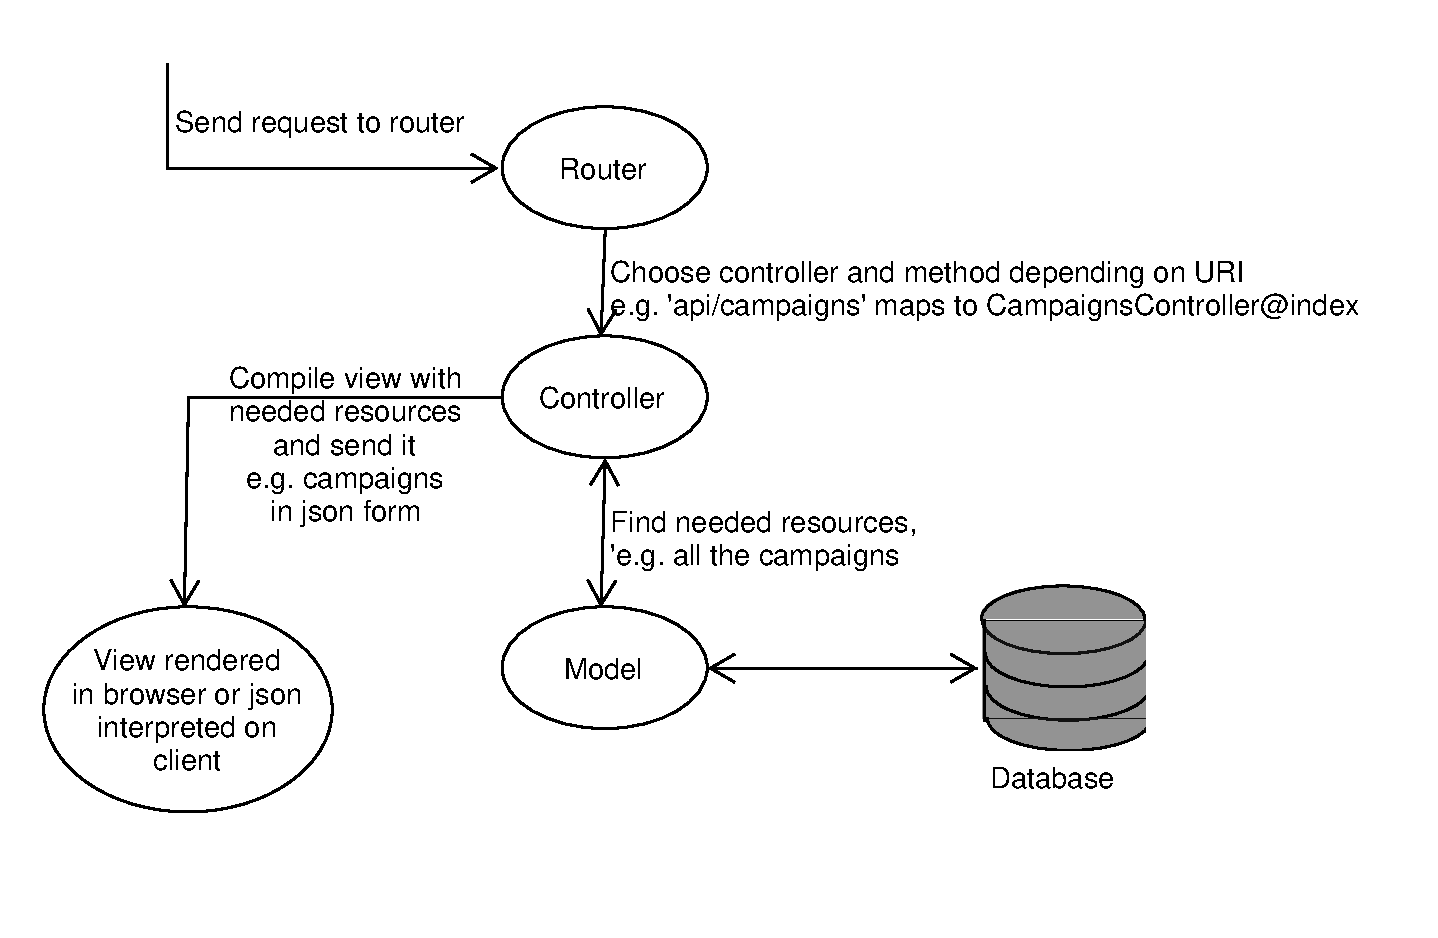
\includegraphics[width=0.7\textwidth]{graphic/architecture/laravel_flow.pdf}
    \caption{An illustration of how a request is traverses through Laravel.}
    \label{fig:laravel_flow}
\end{figure}
\FloatBarrier

Firstly the request is send to the router, which looks at the request URI and determines, depending on the URI, which controller-method should be called, retrieves any parameters captured by wildcards in the URI, and invoke the controller-method with these. It is then the controllers job to fetch the needed models from the database to create the requested view, which in the case of an API route will be a JSON response of the given models. The JSON response will then be interpreted by the Android client and the requested information will be shown to the user. 

\subsubsection{Directing Traffic}
\label{ssub:directing_traffic}
To enable the Laravel framework in the first place we need to direct the traffic to our server from a requested URL to the entry point for the Laravel framework, and there also is the problem that we as mentioned in \secref{sec:server} need to map four different server names to two different sites, namely the production site and the development site. To solve these problems we utilize NGINX. NGINX allows us to specify what is called virtual servers, which allows a single server to listen on different ports, but also allows us to serve different sites depending on the requested server name. Each virtual server has a list of server names associated to them, which is used to determine if the virtual server should handle the request or not, e.g. if a request is made to the URL, \mono{prod.local.element67.dk/api/campaigns}, the virtual server with the server name \mono{prod.local.element67.dk} in its list should handle it. 
Besides the server names, we can specify how the virtual server should process different requests. We can amongst other things specify where to look for the documents to serve by setting the document root or specify that the traffic always should be directed to the entry point for the Laravel framework, namely \mono{index.php}. 
\\\\
An example of how a request to \mono{prod.local.element67.dk/api/campaigns} is handled by our NGINX setup can be seen in \figref{fig:NGINX_workflow}. NGINX will when receiving such a request try to decide, which virtual server should handle the request. In our configuration we have a virtual server defined, which has the server names \mono{prod.local.element67.dk} and \mono{prod.global.element67.dk} attached to it. Therefore NGINX will choose this virtual server. Note that the document root is set to \mono{/var/www/datacollection-prod/public} in the configuration of this virtual server as in \figref{fig:NGINX_workflow}.
\\\\ %Should we mention the document root
Now the server knows what server it should utilize, however it should also determine how the requested URL should be served. For this purpose we can define what is called location directives inside the configuration file of the virtual server. A location directive consists of a rule to match the requested URI, as well as a body containing a strategy or further configuration of how to handle the request. NGINX will then decide which location directive's strategy should be used by finding the best matching location rule. In our configuration for the production server we have defined two different location directives, shown as \emph{location 1} and \emph{location 2} in \figref{fig:NGINX_workflow}. \emph{Location 1}'s rule describes the most general matcher possible, namely \mono{'/'}, and it will therefore act as a fall-back for all requests, whereas the second location is more specific with the rule, \mono{'\textasciitilde ~ \textbackslash .php'}, which is a regular expression rule (defined by the tilde prefix), that will match all requests made to PHP files. 
\\
\begin{figure}[!htbp]
    \centering
    \includegraphics[width=0.7\textwidth]{graphic/architecture/NGINX_workflow.pdf}
    \caption{An example of how a request could be handled by NGINX with our configuration.}
    \label{fig:NGINX_workflow}
\end{figure}
\FloatBarrier

The configuration inside the two locations also vary. \emph{Location 2} will try to handle the request with the following strategies. 
\begin{enumerate}
    \setlength\itemsep{-0.2em}

	\item Try to statically serve the file corresponding to the requested URI, e.g.
	\\\mono{/var/www/datacollection-prod/public/api/campaigns}
	
    \item If that is not possible try to serve an \mono{index.php} file located in the folder corresponding to the URI, e.g.
    \\\mono{/var/www/datacollection-prod/public/api/campaigns/index.php}

	\item If none of the above options exist we will internally redirect the request to the \mono{index.php} located at the root, e.g.
	\\\mono{/var/www/datacollection-prod/public/index.php}
\end{enumerate}

In the second and third of these cases we are dealing with PHP files and NGINX will in this case use \emph{location 2} as the most specific matching location directive. The body of \emph{location 2} then specifies that the request along with the file path to the file to be served should be sent to the PHP interpreter. 

% https://www.digitalocean.com/community/tutorials/how-to-install-laravel-with-an-nginx-web-server-on-ubuntu-14-04
% https://www.digitalocean.com/community/tutorials/understanding-nginx-server-and-location-block-selection-algorithms
% http://nginx.org/en/docs/http/request_processing.html

